\documentclass{article}

% if you need to pass options to natbib, use, e.g.:
\PassOptionsToPackage{numbers, compress}{natbib}
% before loading nips_2016
%
% to avoid loading the natbib package, add option nonatbib:
% \usepackage[nonatbib]{nips_2016}

% \usepackage{nips_2016}

% to compile a camera-ready version, add the [final] option, e.g.:
\usepackage[final]{nips_2016}

\usepackage[utf8]{inputenc} % allow utf-8 input
\usepackage[T1]{fontenc}    % use 8-bit T1 fonts
\usepackage{hyperref}       % hyperlinks
\usepackage{url}            % simple URL typesetting
\usepackage{booktabs}       % professional-quality tables
\usepackage{amsfonts}       % blackboard math symbols
\usepackage{nicefrac}       % compact symbols for 1/2, etc.
\usepackage{microtype}      % microtypography
\usepackage{subcaption}
\usepackage{amsmath}

% Figures
\usepackage{graphicx}
\graphicspath{ {../images/} }

\title{Artistic Style Transfer for Music Data}

% The \author macro works with any number of authors. There are two
% commands used to separate the names and addresses of multiple
% authors: \And and \AND.
%
% Using \And between authors leaves it to LaTeX to determine where to
% break the lines. Using \AND forces a line break at that point. So,
% if LaTeX puts 3 of 4 authors names on the first line, and the last
% on the second line, try using \AND instead of \And before the third
% author name.

\author{
  Patrick~Coleman, David~Penco, Adam~Porisky \\
  Department of Computer Science\\
  University of British Columbia\\
  \texttt{\{padsterpat, dpenco1, adam.porisky\}@gmail.com} \\
}

\begin{document}
\bibliographystyle{plain}

\maketitle

\begin{abstract}
  Recent work in the area of deep learning demonstrates that for 2-D image data, style and content can be learned independently using convolutional neural networks (CNNs) . The neural representation of style and content for two different images can be combined to generate a new image with the content of one image shown in the style of the other. We hypothesize that this method can be applied to music data to achieve a similar effect. Standard visual representations such as spectrograms or mel-frequency cepstrum coefficients (MFCCs) represent sound data in two dimensions, just like images. We directly apply the neural style transfer algorithm to these sound images and transform the result back into audio to generate new sounds with the content of one song and the genre or style of another. In addition, different loss functions that exploit the inherent structure of sound data are explored in an attempt to improve performance. 
\end{abstract}

\section{Introduction}

The application of machine learning principles to artistic or musical data is a unique and ongoing challenge. Machine learning is a powerful tool when it comes to classification of music and other forms of artistic media. Specifically, it is well-documented that deep learning and convolutional neural networks (CNN) allow for feature identification and subsequent categorization of audio content \citep{feng2014, Li2010}. However, a more difficult challenge exists in generating new, compelling artistic content. Projects such as DeepDream, artistic style transfer \citep{Gatys2015}, and NSynth by Magenta \citep{nsynth2017}, are all examples of recent endeavours in this field.

Recent work done by Gatys et al. \citep{Gatys2015} demonstrates that for 2D image data, style and content can be learned independently using CNNs. The activations from two networks, one trained on the input style image and one trained on the input content image, can be used to reconstruct a new output image. This new image preserves the global arrangement and layout of the content image, but with the appearance of the style input image. We suggest that this method can also be applied to music data to achieve a similar effect. We use standard visual representations such as spectrograms or mel-frequency cepstrum coefficients (MFCCs) to represent sound data in a format that is compatible with the neural style transfer algorithm. We then apply the neural style transfer algorithm to these sound images. Transforming the output back into audio generates a new sound file with the content of one song and the genre or style of another.

The loss function implemented by Gatys et al. is a combination of squared-error loss between the feature representations of the output image and the content image, and mean-squared distance between the values of the Gram matrices of the output image and style image \citep{Gatys2015}. To take advantage of the inherent structure that exists within spectrograms and MFCCs, we adjusted the loss functions for the CNNs used to train on the style and content images. We implemented a new loss function based on autocorrelations between horizontal and vertical pixels in an attempt to represent timing and harmonic patterns that exist in the audio data.

In section 3 we describe a method for converting audio data into a form that is compatible with the existing neural style transfer algorithm. We also propose a new loss function capable of yielding better output spectrograms. In section 4 we quantitatively compare the performance of the neural style transfer on audio data for different preprocessing steps and loss functions.


\section{Related Work}

Our work builds upon the neural style transfer implemented by Gatys et al. The authors reconstructed photographs in the style of various well-known pieces of art \citep{Gatys2015}. They discovered that, to an extent, the style and content of an image are separable. By training CNNs with specific feature spaces it is possible to independently learn the style and content of input images. They reconstruct a new image based on the network responses in specific layers for both the style and content images jointly. This results in an output image preserving the arrangement of one image, but with the texture and style of another. The two components are built into the loss function as distinct terms, allowing emphasis of style and content to be varied independently. These parameters are tuned by choosing the most visually appealing result. The applications investigated by the authors are limited to visual forms of media like paintings and photographs. We expand on their framework by modifying it and applying it to audio genre transfer tasks.

Representing sound data in a way that is usable by the neural style transfer algorithm is a key component in our work. As such, we investigated different features that could be used. Tzanetakis et al. propose sets of features to represent texture, rhythmic structure, and instrumentation for the purpose of genre classification \citep{Tzanetakis2001}. Audio data is divided into analysis windows from which features are caluclated, including centroid, rolloff, flux, zero-crossings, and energy. Other features included the mel-frequency cepstral coefficients (MFCCs) and autocorrelations of processed signals. MFCCs have proven to be especially useful in speech recognition tasks. Using these feature sets, each genre is modelled as a multivariate Gaussian and new audio is classified using standard Gaussian classification. Though our ultimate goal is not genre classification, selecting meaningful features that represent the audio in a way that is compatible with the neural style transfer algorithm is an important step.

The work done by Choi et al. also focusses on genre classification, but provides valuable insight into sound representation as well \citep{Choi2016}. The authors converted their audio clips into log-amplitude mel-spectrograms, stating that doing so outperforms standard MFCCs and linear-amplitude mel-spectrograms for genre classification tasks. They compared the performance of convolutional recurrent neural networks (CRNN) with three CNNs of varying structure in both memory-controlled and computation-controlled experiments. According to their results, CRNNs outperform CNNs with 2D convolution kernels when limited to the same number of parameters, but computation using the 2D convolution kernels is faster.

\section{Applying Neural Style Transfer for Audio Data}

\textbf{Dataset.} \hspace{0.25cm} The dataset used in this paper is the Marsyas GTZAN genre collection. It consists of 1000 audio tracks with a length of 30 seconds each. The tracks are separated into 10 genres, each genre having 100 tracks. All of the tracks are recorded in 22050Hz Mono 16-bit audio. The data was originally collected and used by Tzanetakis et al. for genre classification, but has since been made publicly available \citep{Tzanetakis2002}. We trimmed the audio to 10 second clips and applied a bandpass filter as part of a preprocessing step. We chose 10 seconds because it reduces the size of the data for computation purposes, and is still long enough to possess enough characteristic features to be recognized for a particular genre.

\textbf{Network Architecture.} \hspace{0.25cm} We implemented the same machine learning framework as the neural style transfer. The network is based on the 19 layer VGG-Network, a convolutional neural network intended to be used on 2D image data \citep{Simonyan2014}. It is important to note that the weights used for the VGG-Network are pre-trained the ImageNet database \citep{Russ2014}. Features are acquired from the 16 convolutional layers and 5 pooling layers, while ignoring the fully connected layers. More information on the configuration of the network can be seen in \citep{Gatys2015}.

\textbf{2D Audio Representation.} \hspace{0.25cm} Spectrograms and MFCCs are two methods by which audio data can be represented as a two dimensional array. A spectrogram is a plot of the intensity of the short-time Fourier transform (STFT). Sound data is first sectioned into overlapping windows. The Fourier transform is applied to each window, and the results are output as a vertical line showing the intensity at different frequencies. The transform is applied to all of the windows, and the output vertical lines are arranged chronologically. This results in an intensity plot with the horizontal axis representing time, and the vertical axis representing frequency. MFCC plots are also short-term, spectral based features and can be interpreted as a spectrogram with additional processing. To obtain MFCC features, we take the logarithm of the amplitude from the spectorgram, map the results to the mel scale, and then perform a discrete cosine transform \citep{Logan2000}. The mel scale accounts for the difference between actual frequency and perceived pitch. Like the spectrogram, the resulting image plots frequency as a function of time. An example of the spectrogram and MFCCs for the same sound clip is shown in Figure 1.

\textbf{2D Audio Representation.} \hspace{0.25cm} Spectrograms and MFCCs are two methods by which audio data can be represented as a two dimensional array. A spectrogram is a plot of the intensity of the short-time Fourier transform (STFT). Sound data is first sectioned into overlapping windows. The Fourier transform is applied to each window, and the results are output as a vertical line showing the intensity at different frequencies. The transform is applied to all of the windows, and the output vertical lines are arranged chronologically. This results in an intensity plot with the horizontal axis representing time, and the vertical axis representing frequency. MFCC plots are also short-term, spectral based features and can be interpreted as a spectrogram with additional processing. To obtain MFCC features, we take the logarithm of the amplitude from the spectrogram, map the results to the mel scale, and then perform a discrete cosine transform \citep{Logan2000}. The mel scale accounts for the difference between actual frequency and perceived pitch. Like the spectrogram, the resulting image plots frequency as a function of time. An example of the spectrogram and MFCCs for the same sound clip is shown in Figure 1.

\begin{figure}[h]
\begin{subfigure}{\textwidth}
  \centering
  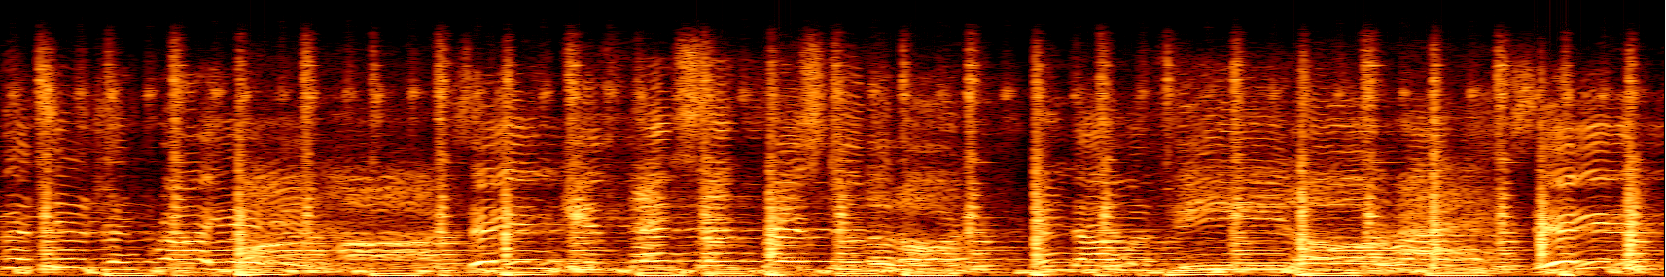
\includegraphics[width = \textwidth]{spec_example}
  \caption{}
\end{subfigure}
 \begin{subfigure}{\textwidth}
  \centering
  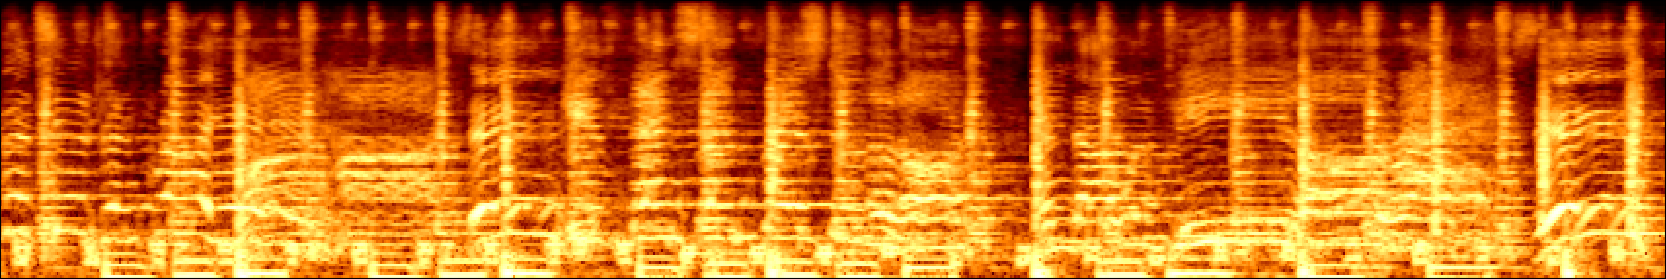
\includegraphics[width = \textwidth]{mel_example}
  \caption{}
\end{subfigure}
\caption{a) Spectrogram transformation of reggae audio clip b) MFCC transformation of reggae audio clip}
\end{figure}

\textbf{Loss Function.} \hspace{0.25cm} The original Neural style transfer paper minimized the following loss functions, for generated image features $F$, content features $P$ and style features $A$:
\begin{align*}
\mathcal{L}_{content}(\text{layer } l) &= \frac{1}{2} \sum_{i, j} (F_{i, j}^{l} - P_{i, j}^{l})^2 \\
\mathcal{L}_{style} &= \sum_l \frac{1}{4N_l^2M_l^2}\sum_{i,j}(G_{i,j}^l(F) - G_{i,j}^l(A))^2
\end{align*}
where we denote the Gram matrix for layer $l$ by $G_{i,j}^l(X) = \sum_k X_{i,k}^l X_{j,k}^l$. 

In this paper, we introduce two new loss functions to minimize that try to capture information properties more useful in the audio domain - specifically, beat and harmonic frequencies. In the context of a spectrogram, the beat pattern can be thought of as how well the signal power correlates with a delayed version of itself.  The music should have a much stronger correlation when delayed the length of a beat, compared to a delay of a shorter length. This is captured by the row-wise autocorrelation for each frequency across time. Similarly, the power strength within a column of the spectrogram captures the harmonics present in the instruments of a song. By matching column autocorrelation, resulting audio should have similar harmonic structure to that of what it is matching.

Mathematically we can define these two properties by the row- and column-wise autocorrelations within the feature matrices. Given image features $F$ as above, we can define to more loss functions by matching its row- and column-wise autocorrelations to the style image:
\begin{align*}
\mathcal{L}_{row^\star} &= \frac{1}{MN} (R^\star(F) - R^\star(A))^2 \\
R^\star(A)_{:,j} &= A_{i,:} \star A_{i,:} \text{ the row autocorrelation, i.e.} \\
R^\star(A)_{i,j} &= \sum_k a_{i,k}a_{i,k-j} \\
\mathcal{L}_{column^\star} &= \frac{1}{MN} (C^\star(F) - C^\star(A))^2 \\
C^\star(A)_{:,j} &= A_{:,j} \star A_{:,j} \text{ the column autocorrelation, i.e.} \\
C^\star(A)_{i,j} &= \sum_k a_{k,j}a_{k-i,j} \\
\end{align*}

The final loss function was then a weighted sum of all four components:
$$
\mathcal{L}_{total} = \alpha \mathcal{L}_{content} + \beta \mathcal{L}_{style} + w_{row} \mathcal{L}_{row^\star} + w_{col} \mathcal{L}_{column^\star}
$$
For this paper, we ran with weights $\alpha = 1\times10^{-3}, \beta = 2\times10^{5}, w_{col} = w_{row} = 1\times10^{-9}$

Note that autocorrelation of a vector is equivalent to convolution with its own reversal, so easy to include within any system that runs convolutional neural networks.

\section{Experiments}

\subsection{Experimental Setup}

To test the algorithm we selected one content audio clip and one style audioclip from the Marsyas GTZAN genre collection database. We chose content and style from two distinct genres to exaggerate any differences. For the results shown below, the content audio is from a song classified in the rock genre, while the style audio is from a song classified in the reggae genre. Spectrograms for the two audio clips are shown in Figure 2.

\begin{figure}[h]
\begin{subfigure}{\textwidth}
  \centering
  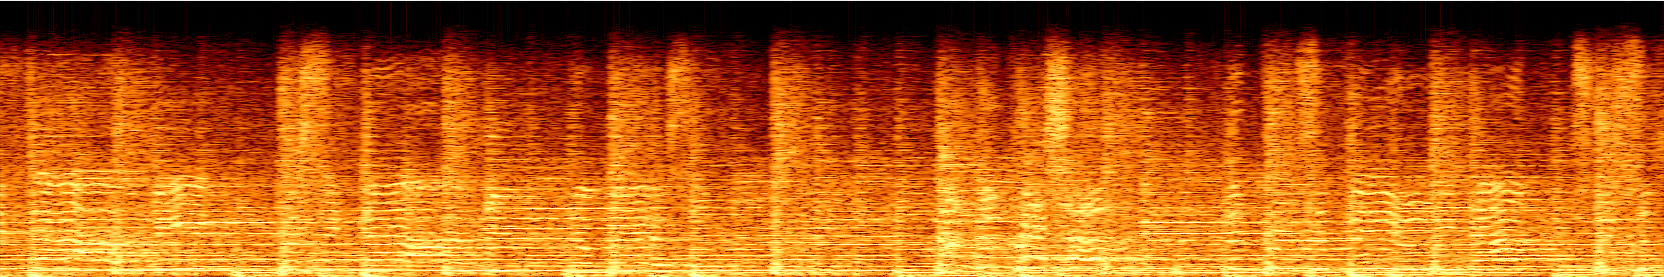
\includegraphics[width = \textwidth]{content_spec}
  \caption{}
\end{subfigure}
\begin{subfigure}{\textwidth}
  \centering
  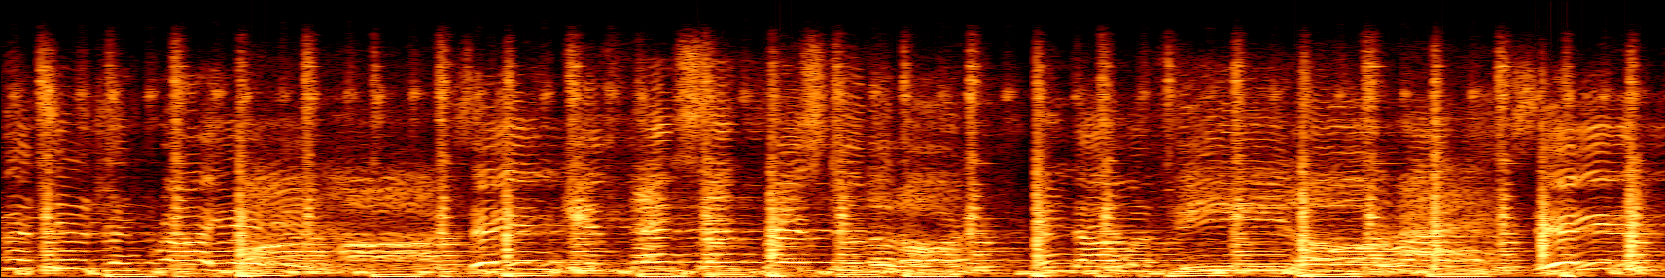
\includegraphics[width = \textwidth]{style_spec}
  \caption{}
\end{subfigure}
\caption{Spectrograms of .wav files for the a) content clip b) style clip}
\end{figure}

Once our audio data is converted into a 2D form that is compatible with the neural style transfer code, the style transfer is applied. Gradient descent is performed on a white noise image with a goal of matching the feature responses as defined by our loss function. We implemented a different number of iterations for the two different formats that we used as inputs. For spectrograms gradient descent was performed for 25 iterations, while for MFCCs 40 iterations were performed. This is because spectrograms have a higher resolution and require more time per iteration.

Code implementing the transfer (and all other stages of processing) was written in Python using the Lasagne and Theano libraries. It is available at \url{https://github.com/padster/AudioStyle}. Results were obtained running on AWS GPU instances (ANY OTHER INFO ON GPU? IE. HARWARE SPECS), taking approximately 10 minutes to complete a transfer. 

\subsection{Results}

HERE: As part of our experiment did we perform style transfer on both spectrograms and MFCCs? Quantitatively describe difference between the two. (Include justification of our selection if we only implemented one).

Discuss the results from original neural transfer loss function

\begin{figure}[!h]
\begin{subfigure}{\textwidth}
  \centering
  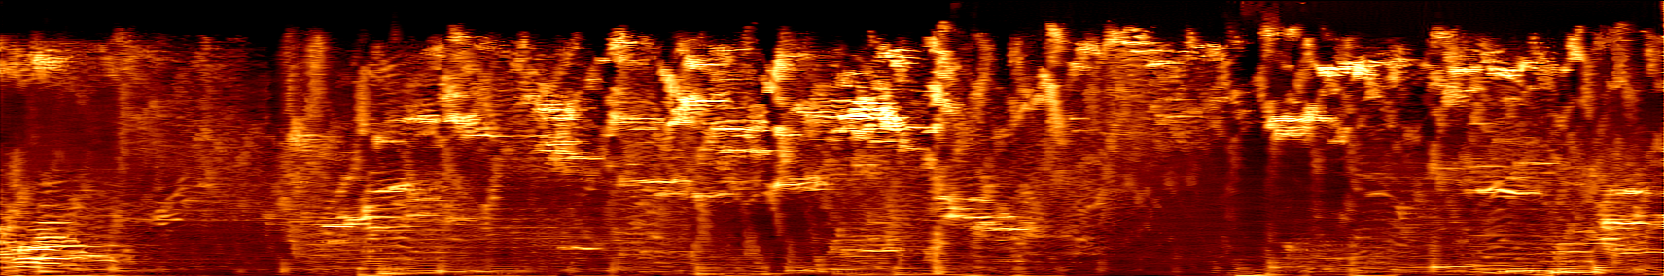
\includegraphics[width = \textwidth]{out1_spec}
  \caption{}
\end{subfigure}
\begin{subfigure}{\textwidth}
  \centering
  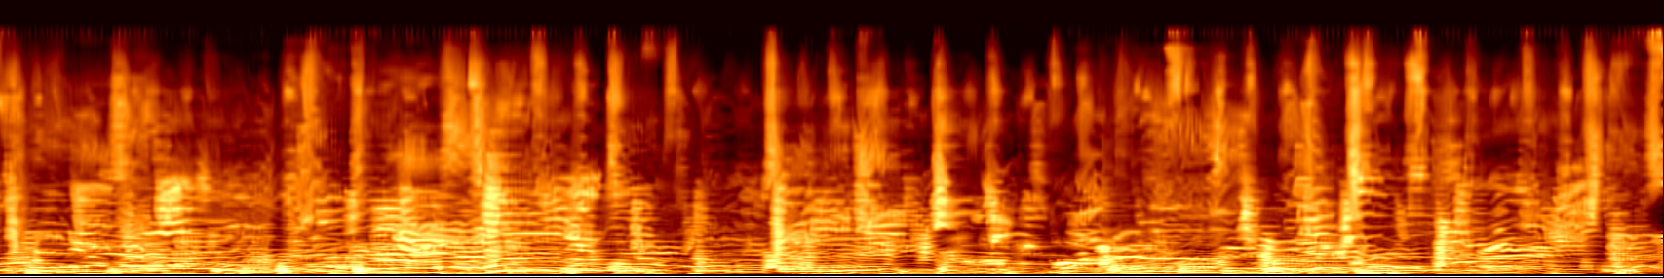
\includegraphics[width = \textwidth]{out2_spec}
  \caption{}
\end{subfigure}
\begin{subfigure}{\textwidth}
  \centering
  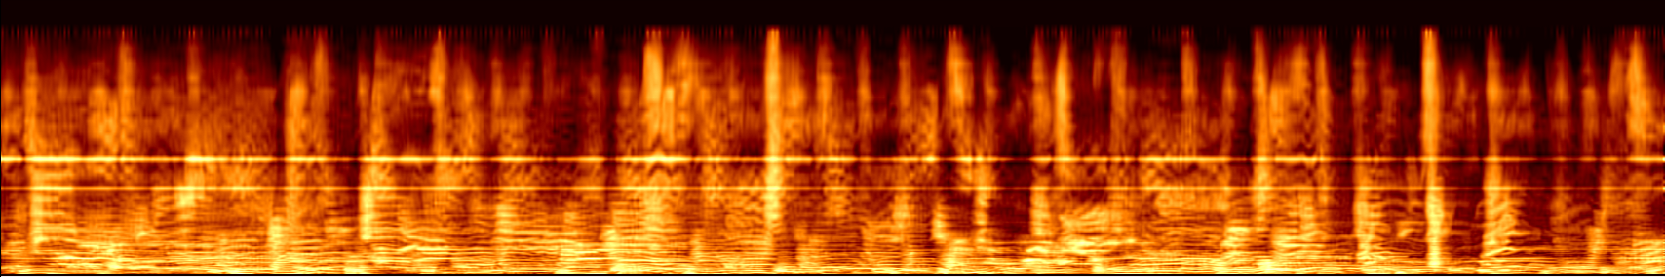
\includegraphics[width = \textwidth]{out3_spec}
  \caption{}
\end{subfigure}
\begin{subfigure}{\textwidth}
  \centering
  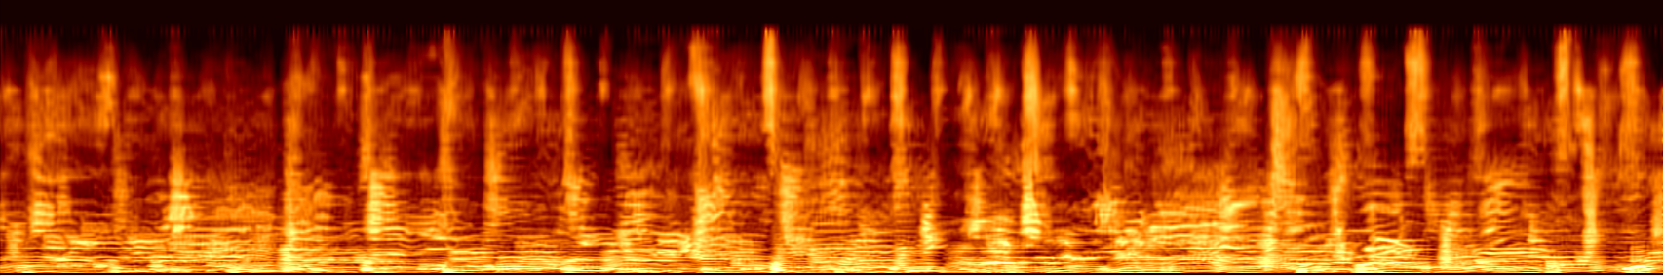
\includegraphics[width = \textwidth]{out4_spec}
  \caption{}
\end{subfigure}
\caption{Output spectrograms after style transfer using a) original loss function b) MFCC transform with original loss function c) MFCC transform with row autocorrelation added to loss function d) MFCC transform with row and column autocorrelation added to loss function}
\end{figure}

Discuss the results from using autocorrelation loss function

\begin{figure}[!h]
\begin{subfigure}{\textwidth}
  \centering
  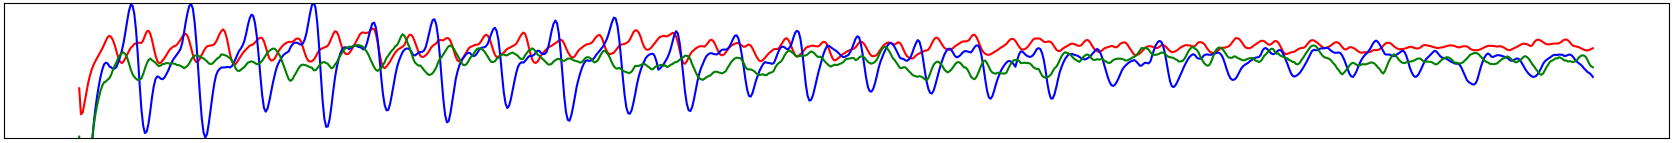
\includegraphics[width = \textwidth]{row_ac_mfcc_input}
  \caption{}
\end{subfigure}
\begin{subfigure}{\textwidth}
  \centering
  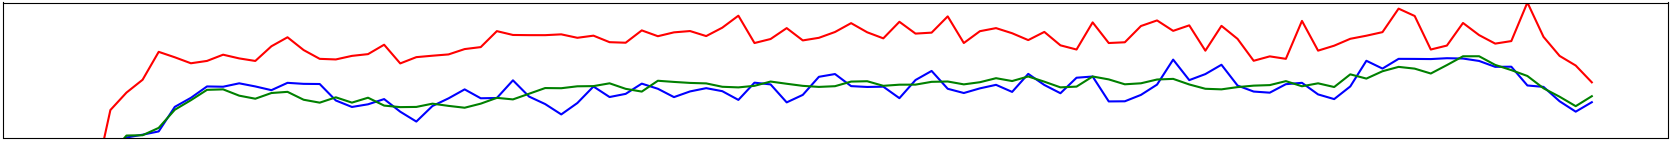
\includegraphics[width = \textwidth]{col_ac_mfcc_input}
  \caption{}
\end{subfigure}
\begin{subfigure}{\textwidth}
  \centering
  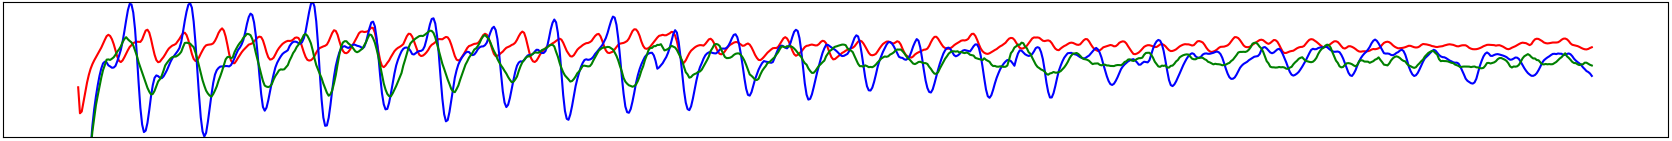
\includegraphics[width = \textwidth]{row_ac_input}
  \caption{}
\end{subfigure}
\begin{subfigure}{\textwidth}
  \centering
  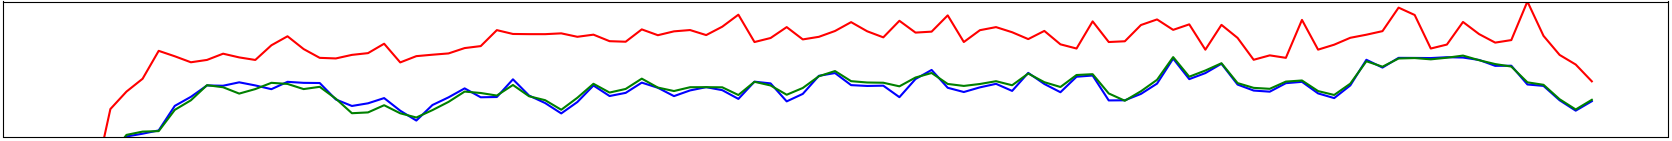
\includegraphics[width = \textwidth]{col_ac_input}
  \caption{}
\end{subfigure}
\caption{Autocorrelation plots. Red, blue, and green lines represent the content, style, and output images respectively. a) Row autocorrelation for MFCC transformation. b) Column autocorrelation for MFCC transformation. c) Row autocorrelation for MFCC transformation with updated loss function. d) Column autocorrelation for MFCC transformation with updated loss function.}
\end{figure}

\section{Discussion and Conclusion}

Did we get satisfactory results from our experiments?

Potential problems associated with out method

One existing challenge facing generative models is evaluation. It is easy to evaluate performance when categorizing art by style, or genre. Properly categorized test cases represent good performance, while misclassification is an example of poor performance. However, evaluation of performance becomes significantly more challenging when considering the output of generative models. Whether or not the result looks like art or sounds like music is typically subjective. As such, there exists a need to develop objective and quantitative performance measures for generative tasks.

\bibliography{CPSC540_FinalReport}

\end{document}

END

%% NIPS style suggestions

\section{General formatting instructions}
\label{gen_inst}

The text must be confined within a rectangle 5.5~inches (33~picas)
wide and 9~inches (54~picas) long. The left margin is 1.5~inch
(9~picas).  Use 10~point type with a vertical spacing (leading) of
11~points.  Times New Roman is the preferred typeface throughout, and
will be selected for you by default.  Paragraphs are separated by
\nicefrac{1}{2}~line space (5.5 points), with no indentation.

The paper title should be 17~point, initial caps/lower case, bold,
centered between two horizontal rules. The top rule should be 4~points
thick and the bottom rule should be 1~point thick. Allow
\nicefrac{1}{4}~inch space above and below the title to rules. All
pages should start at 1~inch (6~picas) from the top of the page.

For the final version, authors' names are set in boldface, and each
name is centered above the corresponding address. The lead author's
name is to be listed first (left-most), and the co-authors' names (if
different address) are set to follow. If there is only one co-author,
list both author and co-author side by side.

Please pay special attention to the instructions in Section \ref{others}
regarding figures, tables, acknowledgments, and references.

\section{Headings: first level}
\label{headings}

All headings should be lower case (except for first word and proper
nouns), flush left, and bold.

First-level headings should be in 12-point type.

\subsection{Headings: second level}

Second-level headings should be in 10-point type.

\subsubsection{Headings: third level}

Third-level headings should be in 10-point type.

\paragraph{Paragraphs}

There is also a \verb+\paragraph+ command available, which sets the
heading in bold, flush left, and inline with the text, with the
heading followed by 1\,em of space.

\section{Citations, figures, tables, references}
\label{others}

These instructions apply to everyone.

\subsection{Citations within the text}

The \verb+natbib+ package will be loaded for you by default.
Citations may be author/year or numeric, as long as you maintain
internal consistency.  As to the format of the references themselves,
any style is acceptable as long as it is used consistently.

The documentation for \verb+natbib+ may be found at
\begin{center}
  \url{http://mirrors.ctan.org/macros/latex/contrib/natbib/natnotes.pdf}
\end{center}
Of note is the command \verb+\citet+, which produces citations
appropriate for use in inline text.  For example,
\begin{verbatim}
   \citet{hasselmo} investigated\dots
\end{verbatim}
produces
\begin{quote}
  Hasselmo, et al.\ (1995) investigated\dots
\end{quote}

If you wish to load the \verb+natbib+ package with options, you may
add the following before loading the \verb+nips_2016+ package:
\begin{verbatim}
   \PassOptionsToPackage{options}{natbib}
\end{verbatim}

If \verb+natbib+ clashes with another package you load, you can add
the optional argument \verb+nonatbib+ when loading the style file:
\begin{verbatim}
   \usepackage[nonatbib]{nips_2016}
\end{verbatim}

As submission is double blind, refer to your own published work in the
third person. That is, use ``In the previous work of Jones et
al.\ [4],'' not ``In our previous work [4].'' If you cite your other
papers that are not widely available (e.g., a journal paper under
review), use anonymous author names in the citation, e.g., an author
of the form ``A.\ Anonymous.''

\subsection{Footnotes}

Footnotes should be used sparingly.  If you do require a footnote,
indicate footnotes with a number\footnote{Sample of the first
  footnote.} in the text. Place the footnotes at the bottom of the
page on which they appear.  Precede the footnote with a horizontal
rule of 2~inches (12~picas).

Note that footnotes are properly typeset \emph{after} punctuation
marks.\footnote{As in this example.}

\subsection{Figures}

All artwork must be neat, clean, and legible. Lines should be dark
enough for purposes of reproduction. The figure number and caption
always appear after the figure. Place one line space before the figure
caption and one line space after the figure. The figure caption should
be lower case (except for first word and proper nouns); figures are
numbered consecutively.

You may use color figures.  However, it is best for the figure
captions and the paper body to be legible if the paper is printed in
either black/white or in color.
\begin{figure}[h]
  \centering
  \fbox{\rule[-.5cm]{0cm}{4cm} \rule[-.5cm]{4cm}{0cm}}
  \caption{Sample figure caption.}
\end{figure}

\subsection{Tables}

All tables must be centered, neat, clean and legible.  The table
number and title always appear before the table.  See
Table~\ref{sample-table}.

Place one line space before the table title, one line space after the
table title, and one line space after the table. The table title must
be lower case (except for first word and proper nouns); tables are
numbered consecutively.

Note that publication-quality tables \emph{do not contain vertical
  rules.} We strongly suggest the use of the \verb+booktabs+ package,
which allows for typesetting high-quality, professional tables:
\begin{center}
  \url{https://www.ctan.org/pkg/booktabs}
\end{center}
This package was used to typeset Table~\ref{sample-table}.

\begin{table}[t]
  \caption{Sample table title}
  \label{sample-table}
  \centering
  \begin{tabular}{lll}
    \toprule
    \multicolumn{2}{c}{Part}                   \\
    \cmidrule{1-2}
    Name     & Description     & Size ($\mu$m) \\
    \midrule
    Dendrite & Input terminal  & $\sim$100     \\
    Axon     & Output terminal & $\sim$10      \\
    Soma     & Cell body       & up to $10^6$  \\
    \bottomrule
  \end{tabular}
\end{table}

\section{Final instructions}

Do not change any aspects of the formatting parameters in the style
files.  In particular, do not modify the width or length of the
rectangle the text should fit into, and do not change font sizes
(except perhaps in the \textbf{References} section; see below). Please
note that pages should be numbered.

\section{Preparing PDF files}

Please prepare submission files with paper size ``US Letter,'' and
not, for example, ``A4.''

Fonts were the main cause of problems in the past years. Your PDF file
must only contain Type 1 or Embedded TrueType fonts. Here are a few
instructions to achieve this.

\begin{itemize}

\item You should directly generate PDF files using \verb+pdflatex+.

\item You can check which fonts a PDF files uses.  In Acrobat Reader,
  select the menu Files$>$Document Properties$>$Fonts and select Show
  All Fonts. You can also use the program \verb+pdffonts+ which comes
  with \verb+xpdf+ and is available out-of-the-box on most Linux
  machines.

\item The IEEE has recommendations for generating PDF files whose
  fonts are also acceptable for NIPS. Please see
  \url{http://www.emfield.org/icuwb2010/downloads/IEEE-PDF-SpecV32.pdf}

\item \verb+xfig+ "patterned" shapes are implemented with bitmap
  fonts.  Use "solid" shapes instead.

\item The \verb+\bbold+ package almost always uses bitmap fonts.  You
  should use the equivalent AMS Fonts:
\begin{verbatim}
   \usepackage{amsfonts}
\end{verbatim}
followed by, e.g., \verb+\mathbb{R}+, \verb+\mathbb{N}+, or
\verb+\mathbb{C}+ for $\mathbb{R}$, $\mathbb{N}$ or $\mathbb{C}$.  You
can also use the following workaround for reals, natural and complex:
\begin{verbatim}
   \newcommand{\RR}{I\!\!R} %real numbers
   \newcommand{\Nat}{I\!\!N} %natural numbers
   \newcommand{\CC}{I\!\!\!\!C} %complex numbers
\end{verbatim}
Note that \verb+amsfonts+ is automatically loaded by the
\verb+amssymb+ package.

\end{itemize}

If your file contains type 3 fonts or non embedded TrueType fonts, we
will ask you to fix it.

\subsection{Margins in \LaTeX{}}

Most of the margin problems come from figures positioned by hand using
\verb+\special+ or other commands. We suggest using the command
\verb+\includegraphics+ from the \verb+graphicx+ package. Always
specify the figure width as a multiple of the line width as in the
example below:
\begin{verbatim}
   \usepackage[pdftex]{graphicx} ...
   \includegraphics[width=0.8\linewidth]{myfile.pdf}
\end{verbatim}
See Section 4.4 in the graphics bundle documentation
(\url{http://mirrors.ctan.org/macros/latex/required/graphics/grfguide.pdf})

A number of width problems arise when \LaTeX{} cannot properly
hyphenate a line. Please give LaTeX hyphenation hints using the
\verb+\-+ command when necessary.

\subsubsection*{Acknowledgments}

Use unnumbered third level headings for the acknowledgments. All
acknowledgments go at the end of the paper. Do not include
acknowledgments in the anonymized submission, only in the final paper.

\section*{References}

References follow the acknowledgments. Use unnumbered first-level
heading for the references. Any choice of citation style is acceptable
as long as you are consistent. It is permissible to reduce the font
size to \verb+small+ (9 point) when listing the references. {\bf
  Remember that you can use a ninth page as long as it contains
  \emph{only} cited references.}
\medskip

\small

[1] Alexander, J.A.\ \& Mozer, M.C.\ (1995) Template-based algorithms
for connectionist rule extraction. In G.\ Tesauro, D.S.\ Touretzky and
T.K.\ Leen (eds.), {\it Advances in Neural Information Processing
  Systems 7}, pp.\ 609--616. Cambridge, MA: MIT Press.

[2] Bower, J.M.\ \& Beeman, D.\ (1995) {\it The Book of GENESIS:
  Exploring Realistic Neural Models with the GEneral NEural SImulation
  System.}  New York: TELOS/Springer--Verlag.

[3] Hasselmo, M.E., Schnell, E.\ \& Barkai, E.\ (1995) Dynamics of
learning and recall at excitatory recurrent synapses and cholinergic
modulation in rat hippocampal region CA3. {\it Journal of
  Neuroscience} {\bf 15}(7):5249-5262.
